\documentclass[12pt,a4paper]{article}
\usepackage[margin=2.2cm]{geometry}
\usepackage{ctex}
\usepackage{amsmath,amssymb,amsfonts}
\usepackage{graphicx}
\usepackage{tikz}
\usetikzlibrary{calc,positioning,arrows.meta,decorations.pathreplacing,matrix,patterns}
\usepackage{booktabs}
\usepackage{enumitem}
\usepackage{xcolor}
\usepackage{tcolorbox}
\usepackage{hyperref}
\usepackage{float}
\usepackage{array}
\usepackage{multirow}
\usepackage{longtable}

\tcbuselibrary{theorems,skins,breakable}

\definecolor{myblue}{RGB}{0,102,204}
\definecolor{myred}{RGB}{204,0,0}
\definecolor{mygreen}{RGB}{0,153,0}
\definecolor{mypurple}{RGB}{128,0,128}
\definecolor{myorange}{RGB}{230,120,0}
\definecolor{lightblue}{RGB}{220,235,255}
\definecolor{lightyellow}{RGB}{255,255,220}
\definecolor{lightgreen}{RGB}{220,255,220}
\definecolor{lightred}{RGB}{255,225,225}
\definecolor{lightpurple}{RGB}{240,225,255}
\definecolor{queencol}{RGB}{255,215,0}
\definecolor{attackcol}{RGB}{255,100,100}

\newtcolorbox{keybox}[1][]{
  colback=lightblue, colframe=myblue,
  fonttitle=\bfseries, title={#1},
  breakable
}

\newtcolorbox{exbox}[1][]{
  colback=lightyellow, colframe=myorange,
  fonttitle=\bfseries, title={#1},
  breakable
}

\newtcolorbox{warnbox}[1][]{
  colback=lightred, colframe=myred,
  fonttitle=\bfseries, title={#1},
  breakable
}

\newtcolorbox{sumbox}[1][]{
  colback=lightgreen, colframe=mygreen,
  fonttitle=\bfseries, title={#1},
  breakable
}

\newtcolorbox{notebox}[1][]{
  colback=lightpurple, colframe=mypurple,
  fonttitle=\bfseries, title={#1},
  breakable
}

\newtcolorbox{stepbox}[1][]{
  colback=white, colframe=myblue!70!black,
  fonttitle=\bfseries, title={#1},
  breakable, left=4mm, right=4mm,
  boxrule=1.2pt
}

\newcommand{\Q}{\textcolor{myred}{\textbf{Q}}}
\newcommand{\bv}[1]{\boldsymbol{#1}}

\title{\Huge\textbf{4$\times$4 皇后问题} \\ \Large 转移矩阵法完整计算过程}
\author{张量网络学习笔记}
\date{}

\begin{document}
\maketitle
\tableofcontents
\newpage

%=============================================================================
\section{问题描述}
%=============================================================================

在 $4\times 4$ 的棋盘上放置 4 个皇后，使得：
\begin{itemize}
  \item 每行恰好 1 个皇后
  \item 每列恰好 1 个皇后
  \item 每条对角线至多 1 个皇后
\end{itemize}

\begin{keybox}[目标]
  通过转移矩阵法，\textbf{从头到尾展示}如何算出解的个数 $Z_4 = 2$。
\end{keybox}

先给出两个解的直观图示：

\begin{center}
\begin{tikzpicture}[scale=0.8]
  % Solution 1
  \node[above] at (2, 4.3) {\textbf{解 1}};
  \foreach \r/\c in {0/1, 1/3, 2/0, 3/2}{
    \fill[queencol!40] (\c, 3-\r) rectangle (\c+1, 4-\r);
  }
  \draw[step=1, thick] (0,0) grid (4,4);
  \foreach \r/\c in {0/1, 1/3, 2/0, 3/2}{
    \node[font=\Large\bfseries] at (\c+0.5, 3.5-\r) {\textcolor{myred}{Q}};
  }
  \foreach \i in {0,...,3}{
    \node[left, font=\small] at (0, 3.5-\i) {行\i};
    \node[below, font=\small] at (\i+0.5, 0) {列\i};
  }
  % Solution 2
  \begin{scope}[xshift=6cm]
  \node[above] at (2, 4.3) {\textbf{解 2}};
  \foreach \r/\c in {0/2, 1/0, 2/3, 3/1}{
    \fill[queencol!40] (\c, 3-\r) rectangle (\c+1, 4-\r);
  }
  \draw[step=1, thick] (0,0) grid (4,4);
  \foreach \r/\c in {0/2, 1/0, 2/3, 3/1}{
    \node[font=\Large\bfseries] at (\c+0.5, 3.5-\r) {\textcolor{myred}{Q}};
  }
  \foreach \i in {0,...,3}{
    \node[left, font=\small] at (0, 3.5-\i) {行\i};
    \node[below, font=\small] at (\i+0.5, 0) {列\i};
  }
  \end{scope}
\end{tikzpicture}
\end{center}

接下来我们将展示，如何通过\textbf{转移矩阵}从零开始推导出这个结果。

%=============================================================================
\section{基本构件}
%=============================================================================

\subsection{占据算符}

每个格点 $\sigma \in \{0, 1\}$，其中 $0$ 表示空，$1$ 表示有皇后。
定义投影算符：
\[
\hat{n}_0 = |0\rangle\langle 0| = \begin{pmatrix} 1 \\ 0 \end{pmatrix}\begin{pmatrix} 1 & 0 \end{pmatrix} = \begin{pmatrix} 1 & 0 \\ 0 & 0 \end{pmatrix}, \quad
\hat{n}_1 = |1\rangle\langle 1| = \begin{pmatrix} 0 \\ 1 \end{pmatrix}\begin{pmatrix} 0 & 1 \end{pmatrix} = \begin{pmatrix} 0 & 0 \\ 0 & 1 \end{pmatrix}
\]

性质：$\hat{n}_0 + \hat{n}_1 = I$，$\hat{n}_0 \hat{n}_1 = 0$。

\subsection{转移矩阵 $A$}

\begin{keybox}[核心构件：$A$ 矩阵]
$A$ 矩阵的元素是算符，作用在物理指标 $\sigma$ 上：
\[
A = \begin{pmatrix} \hat{n}_0 & \hat{n}_1 \\ 0 & \hat{n}_0 \end{pmatrix}
\]
写成三指标张量 $A_{\alpha\beta}(\sigma)$，其中 $\alpha,\beta \in \{0,1\}$ 是 bond 指标，$\sigma \in \{0,1\}$ 是物理指标：
\end{keybox}

展开所有分量：

\begin{center}
\renewcommand{\arraystretch}{1.3}
\begin{tabular}{c|cccc|l}
\toprule
$\sigma$ & $A_{00}(\sigma)$ & $A_{01}(\sigma)$ & $A_{10}(\sigma)$ & $A_{11}(\sigma)$ & 含义 \\
\midrule
$0$ (空) & $1$ & $0$ & $0$ & $1$ & 空格：信号透传 ($\alpha \to \alpha$) \\
$1$ (Q) & $0$ & $1$ & $0$ & $0$ & 皇后：无信号$\to$发出信号 ($0 \to 1$) \\
\bottomrule
\end{tabular}
\end{center}

\begin{notebox}[物理图像]
把 $\alpha$ 看作一条信号线上的状态：
\begin{itemize}[nosep]
  \item $\alpha = 0$：信号线上\textbf{还没有}皇后通过
  \item $\alpha = 1$：信号线上\textbf{已经有}皇后通过
\end{itemize}
$A(\sigma=0)$：空格不改变信号状态 → $A(0) = I$（恒等矩阵）\\
$A(\sigma=1)$：皇后把信号从 $0$ 变为 $1$ → $A_{01}(1) = 1$，其余为零\\
如果信号已经是 $1$，再遇到皇后 → $A_{11}(1) = 0$，链值归零（禁止两个皇后）
\end{notebox}

\subsection{边界向量}

\begin{keybox}[三种边界条件]
\begin{align}
\bv{v}_0 &= (1, 0) \quad \text{--- 约束线的\textbf{起点}：信号初始为 0} \\
\bv{v}_1 &= (0, 1) \quad \text{--- 「恰好 1 个」：要求信号最终变为 1} \\
\bv{v}_2 &= (1, 1) \quad \text{--- 「至多 1 个」：信号 0 或 1 均可}
\end{align}
\end{keybox}

%=============================================================================
\section{一维约束链的收缩}
%=============================================================================

\subsection{什么是「收缩」}

「收缩」就是\textbf{把共享指标求和消掉}。矩阵乘法 $C_{ik} = \sum_j A_{ij} B_{jk}$ 就是对指标 $j$ 的收缩。

对于一条约束链，收缩就是连续矩阵乘法：
\[
f(\sigma_1, \sigma_2, \dots, \sigma_L) = \bv{v}_0 \cdot A(\sigma_1) \cdot A(\sigma_2) \cdots A(\sigma_L) \cdot \bv{v}_{\text{end}}^T
\]

这里 $\bv{v}_0$ 是 $1\times 2$ 行向量，每个 $A(\sigma_i)$ 是 $2\times 2$ 矩阵，$\bv{v}_{\text{end}}$ 是 $2\times 1$ 列向量，最终得到一个\textbf{标量}。

\subsection{行约束示例：第 0 行}

以第 0 行为例，要求恰好放 1 个皇后。设 4 个格点的占据 $(\sigma_0, \sigma_1, \sigma_2, \sigma_3)$，
约束值为：
\[
f_{\text{row}} = \bv{v}_0 \cdot A(\sigma_0) \cdot A(\sigma_1) \cdot A(\sigma_2) \cdot A(\sigma_3) \cdot \bv{v}_1^T
\]

\begin{exbox}[示例 1：$(\sigma_0, \sigma_1, \sigma_2, \sigma_3) = (0, 1, 0, 0)$ --- 列 1 放皇后]
逐步计算：
\begin{align*}
\bv{v}_0 &= (1, 0) & \text{初始：无信号} \\[3pt]
(1,0) \cdot A(0) &= (1,0) \cdot \begin{pmatrix}1&0\\0&1\end{pmatrix} = (1, 0) & \text{列0空：不变} \\[3pt]
(1,0) \cdot A(1) &= (1,0) \cdot \begin{pmatrix}0&1\\0&0\end{pmatrix} = (0, 1) & \text{列1放Q：信号$0\!\to\!1$} \\[3pt]
(0,1) \cdot A(0) &= (0,1) \cdot \begin{pmatrix}1&0\\0&1\end{pmatrix} = (0, 1) & \text{列2空：信号传递} \\[3pt]
(0,1) \cdot A(0) &= (0,1) \cdot \begin{pmatrix}1&0\\0&1\end{pmatrix} = (0, 1) & \text{列3空：信号传递} \\[3pt]
(0,1) \cdot \bv{v}_1^T &= (0,1) \cdot \binom{0}{1} = \textcolor{mygreen}{\boldsymbol{1}} & \text{信号=1，满足!}
\end{align*}
\end{exbox}

\begin{exbox}[示例 2：$(0, 1, 0, 1)$ --- 列 1 和列 3 各放一个皇后]
\begin{align*}
(1,0) \cdot A(0) &= (1, 0) \\
(1,0) \cdot A(1) &= (0, 1) & \text{第一个Q：信号$\to$1} \\
(0,1) \cdot A(0) &= (0, 1) \\
(0,1) \cdot A(1) &= (0,1) \cdot \begin{pmatrix}0&1\\0&0\end{pmatrix} = \textcolor{myred}{(0, 0)} & \text{第二个Q：$A_{11}(1)=0$，被杀死！} \\
(0,0) \cdot \bv{v}_1^T &= \textcolor{myred}{\boldsymbol{0}} & \text{两个Q → 禁止}
\end{align*}
\end{exbox}

\begin{exbox}[示例 3：$(0, 0, 0, 0)$ --- 没有皇后]
\begin{align*}
(1,0) \cdot A(0)^4 &= (1, 0) & \text{全空：信号始终为 0} \\
(1,0) \cdot \bv{v}_1^T &= \textcolor{myred}{\boldsymbol{0}} & \text{$v_1$ 要求信号=1，不满足}
\end{align*}
\end{exbox}

\begin{sumbox}[小结]
$\bv{v}_0 \cdot A(\sigma_1) \cdots A(\sigma_L) \cdot \bv{v}_1^T$ 的值：
\begin{itemize}[nosep]
  \item $=1$：链上恰好有 1 个皇后
  \item $=0$：链上有 0 个或 $\geq 2$ 个皇后
\end{itemize}
如果把 $\bv{v}_1$ 换成 $\bv{v}_2 = (1,1)$，则「至多 1 个」也是合法的（用于对角线约束）。
\end{sumbox}

\subsection{对角线约束示例}

$4\times 4$ 棋盘有 7 条 $\searrow$ 对角线和 7 条 $\nearrow$ 对角线。以主对角线 $\searrow$（经过 $(0,0),(1,1),(2,2),(3,3)$，长度 4）为例：

\[
f_{\text{diag}} = \bv{v}_0 \cdot A(\sigma_{00}) \cdot A(\sigma_{11}) \cdot A(\sigma_{22}) \cdot A(\sigma_{33}) \cdot \bv{v}_2^T
\]

对角线用 $\bv{v}_2 = (1,1)$ 结尾：0 个或 1 个皇后都给 $f=1$，2 个以上给 $f=0$。

%=============================================================================
\section{从约束链到 T 张量}
%=============================================================================

\subsection{约束的方向}

每个格点 $(i,j)$ 被 4 条约束线穿过：
\begin{center}
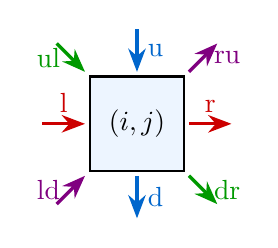
\begin{tikzpicture}[scale=1.2, >=Stealth]
  \fill[lightblue!50] (0,0) rectangle (1,1);
  \draw[thick] (0,0) rectangle (1,1);
  \node at (0.5,0.5) {$(i,j)$};
  % arrows
  \draw[very thick, myblue, ->] (0.5, 1.5) -- (0.5, 1.05) node[midway, right] {u};
  \draw[very thick, myblue, ->] (0.5, -0.05) -- (0.5, -0.5) node[midway, right] {d};
  \draw[very thick, myred, ->] (-0.5, 0.5) -- (-0.05, 0.5) node[midway, above] {l};
  \draw[very thick, myred, ->] (1.05, 0.5) -- (1.5, 0.5) node[midway, above] {r};
  \draw[very thick, mygreen, ->] (-0.35, 1.35) -- (-0.05, 1.05) node[midway, left] {ul};
  \draw[very thick, mygreen, ->] (1.05, -0.05) -- (1.35, -0.35) node[midway, right] {dr};
  \draw[very thick, mypurple, ->] (-0.35, -0.35) -- (-0.05, -0.05) node[midway, left] {ld};
  \draw[very thick, mypurple, ->] (1.05, 1.05) -- (1.35, 1.35) node[midway, right] {ru};
\end{tikzpicture}
\end{center}

\begin{itemize}[nosep]
  \item \textcolor{myblue}{\textbf{u, d}}：列约束（上$\to$下）
  \item \textcolor{myred}{\textbf{l, r}}：行约束（左$\to$右）
  \item \textcolor{mygreen}{\textbf{ul, dr}}：$\searrow$ 对角线约束（左上$\to$右下）
  \item \textcolor{mypurple}{\textbf{ld, ru}}：$\nearrow$ 对角线约束（左下$\to$右上）
\end{itemize}

\subsection{局部 T 张量}

每个格点的 T 张量是 4 条约束线上 $A$ 矩阵元的乘积：

\begin{keybox}[T 张量的构造公式]
\[
T(u,d,l,r,\textit{ul},\textit{dr},\textit{ld},\textit{ru},p) = A_{ud}(p) \cdot A_{lr}(p) \cdot A_{\textit{ul},\textit{dr}}(p) \cdot A_{\textit{ld},\textit{ru}}(p)
\]
其中 $p = \sigma \in \{0,1\}$ 是物理指标，其余 8 个是 bond 指标。
\end{keybox}

由于 $A$ 矩阵只有 3 个非零元（$A_{00}(0)=1, A_{11}(0)=1, A_{01}(1)=1$），
T 张量的非零条件是 4 个因子\textbf{同时}非零：

\begin{itemize}
  \item \textbf{$p=0$（空格）}：每个因子 $A_{\alpha\beta}(0)$ 非零要求 $\alpha=\beta$，
        即 $u\!=\!d,\; l\!=\!r,\; ul\!=\!dr,\; ld\!=\!ru$。\\
        4 个独立的 $\{0,1\}$ 选择 $\to$ $2^4=16$ 个非零元，全为 1。\\
        \textbf{含义}：空格对每条信号线独立透传（有信号就传，没有就不传）。
  \item \textbf{$p=1$（皇后）}：每个因子 $A_{01}(1)$ 非零要求输入$=0$，输出$=1$，
        即 $u\!=\!l\!=\!ul\!=\!ld\!=\!0$，$d\!=\!r\!=\!dr\!=\!ru\!=\!1$。\\
        只有 \textbf{1} 个非零元。\\
        \textbf{含义}：皇后要求所有方向无冲突（输入全0），并向所有方向发出攻击信号（输出全1）。
\end{itemize}

共 $16 + 1 = \textbf{17}$ 个非零元。

%=============================================================================
\section{$4\times 4$ 张量网络}
%=============================================================================

\subsection{网络拓扑}

$4\times 4$ 棋盘上 16 个 T 张量通过 bond 指标连接：

\begin{center}
\begin{tikzpicture}[scale=1.6, >=Stealth,
    site/.style={circle, draw, thick, fill=lightblue!50, minimum size=7mm, inner sep=0pt, font=\scriptsize}]
  % Nodes
  \foreach \i in {0,...,3}{
    \foreach \j in {0,...,3}{
      \node[site] (T\i\j) at (\j, -\i) {$T_{\i\j}$};
    }
  }
  % Horizontal bonds (row constraints, red)
  \foreach \i in {0,...,3}{
    \foreach \j [evaluate=\j as \jn using int(\j+1)] in {0,1,2}{
      \draw[thick, myred] (T\i\j) -- (T\i\jn);
    }
  }
  % Vertical bonds (column constraints, blue)
  \foreach \i [evaluate=\i as \in using int(\i+1)] in {0,1,2}{
    \foreach \j in {0,...,3}{
      \draw[thick, myblue] (T\i\j) -- (T\in\j);
    }
  }
  % SE diagonal bonds (green)
  \foreach \i [evaluate=\i as \in using int(\i+1)] in {0,1,2}{
    \foreach \j [evaluate=\j as \jn using int(\j+1)] in {0,1,2}{
      \draw[thick, mygreen, densely dashed] (T\i\j) -- (T\in\jn);
    }
  }
  % NE diagonal bonds (purple)
  \foreach \i [evaluate=\i as \in using int(\i+1)] in {0,1,2}{
    \foreach \j [evaluate=\j as \jn using int(\j-1)] in {1,2,3}{
      \draw[thick, mypurple, densely dotted] (T\i\j) -- (T\in\jn);
    }
  }
  % Legend
  \node[right, font=\small] at (4.3, 0) {\textcolor{myred}{--- 行约束}};
  \node[right, font=\small] at (4.3, -0.5) {\textcolor{myblue}{--- 列约束}};
  \node[right, font=\small] at (4.3, -1.0) {\textcolor{mygreen}{- - $\searrow$ 对角线}};
  \node[right, font=\small] at (4.3, -1.5) {\textcolor{mypurple}{$\cdots$ $\nearrow$ 对角线}};
\end{tikzpicture}
\end{center}

每条连线代表一个共享的 bond 指标，收缩网络就是对所有 bond 指标求和。

\subsection{边界条件}

每条约束线有一个\textbf{起点}（乘以 $\bv{v}_0$）和一个\textbf{终点}（乘以 $\bv{v}_1$ 或 $\bv{v}_2$）：

\begin{center}
\renewcommand{\arraystretch}{1.2}
\begin{tabular}{l|c|c|c}
\toprule
约束线 & 起点 ($\bv{v}_0$) & 终点 & 数量 \\
\midrule
行 (l/r) & 每行最左的 l & 每行最右的 r，乘 $\bv{v}_1$ & 4 \\
列 (u/d) & 每列最上的 u & 每列最下的 d，乘 $\bv{v}_1$ & 4 \\
$\searrow$ 对角线 (ul/dr) & 起始端的 ul & 终止端的 dr，乘 $\bv{v}_2$ & 7 \\
$\nearrow$ 对角线 (ld/ru) & 起始端的 ld & 终止端的 ru，乘 $\bv{v}_2$ & 7 \\
\bottomrule
\end{tabular}
\end{center}

起点 $\bv{v}_0 = (1,0)$ 意味着该指标固定为 $0$（信号尚未发出）。
终点 $\bv{v}_1 = (0,1)$ 固定为 $1$（要求信号已发出 --- 恰好 1 个皇后）。
终点 $\bv{v}_2 = (1,1)$ 对 $0$ 和 $1$ 都接受（至多 1 个皇后）。

\subsection{分区函数}

把所有 T 张量连接、乘以边界向量后，对所有物理指标 $p_{ij}$ 求和：
\[
\boxed{Z_4 = \sum_{\{p_{ij}\}} \Bigl(\text{收缩所有 bond 指标后的标量值}\Bigr)}
\]

这就是我们要计算的 $4\times 4$ 皇后问题的解数。

%=============================================================================
\section{逐行收缩：计算策略}
%=============================================================================

直接收缩 16 个 9 指标张量非常复杂。实际操作中，我们\textbf{逐行}处理：

\begin{enumerate}
  \item 从第 0 行开始，逐行向下扫描
  \item 每行必须放恰好 1 个皇后（行约束由 $\bv{v}_0 \cdot A^4 \cdot \bv{v}_1$ 保证）
  \item 行内约束在该行处理完毕后自动满足
  \item \textbf{行间传递的信息}：需要记住哪些列/对角线已被占据
\end{enumerate}

\begin{keybox}[行间状态]
处理完第 $i$ 行后，需要记录三组信息传递到第 $i+1$ 行：
\begin{itemize}[nosep]
  \item $C$：已被皇后占据的\textbf{列}集合（列约束 u/d 方向信号）
  \item $D_\searrow$：第 $i+1$ 行中被 $\searrow$ 对角线攻击的列集合
  \item $D_\nearrow$：第 $i+1$ 行中被 $\nearrow$ 对角线攻击的列集合
\end{itemize}
\end{keybox}

\subsection{对角线信号的移位规则}

\begin{warnbox}[关键：对角线信号每行移位]
皇后在 $(i,j)$ 处的 $\searrow$ 对角线攻击到达第 $i+k$ 行时，攻击的是列 $j+k$。
因此 $D_\searrow$ 的信号每过一行\textbf{向右移一格}。

类似地，$\nearrow$ 信号每过一行\textbf{向左移一格}。

用 $A$ 矩阵的语言：空格 $A_{11}(0) = 1$ 表示信号透传，对角线上的信号经过空格后传递到下一行的相邻列。
\end{warnbox}

具体规则：在第 $i$ 行列 $j$ 放皇后后，更新对角线信号：
\begin{align}
D_\searrow^{\text{new}} &= \text{shift\_right}\bigl(D_\searrow^{\text{old}} \cup \{j\}\bigr)
  = \{k+1 : k \in D_\searrow^{\text{old}} \cup \{j\},\; k+1 < 4\} \\
D_\nearrow^{\text{new}} &= \text{shift\_left}\bigl(D_\nearrow^{\text{old}} \cup \{j\}\bigr)
  = \{k-1 : k \in D_\nearrow^{\text{old}} \cup \{j\},\; k-1 \geq 0\}
\end{align}

%=============================================================================
\section{完整计算：逐行展开}
%=============================================================================

下面我们\textbf{逐行}展开全部计算过程。状态记为 $(C, D_\searrow, D_\nearrow)$。

%--- Row 0 ---
\subsection{第 0 行}

\begin{stepbox}[第 0 行：初始状态]
初始状态：$(C=\emptyset,\; D_\searrow=\emptyset,\; D_\nearrow=\emptyset)$，计数 $= 1$

可用列 $= \{0,1,2,3\} \setminus C \setminus D_\searrow \setminus D_\nearrow = \{0,1,2,3\}$

所有 4 列都可以放皇后。
\end{stepbox}

在每一列放皇后后的新状态：

\begin{center}
\renewcommand{\arraystretch}{1.4}
\begin{tabular}{c|c|c|c|c|l}
\toprule
编号 & 皇后位置 & 新 $C$ & 新 $D_\searrow$ & 新 $D_\nearrow$ & 计算过程 \\
\midrule
S1 & 列 0 & $\{0\}$ & $\{1\}$ & $\emptyset$ & $D_\searrow$: $\{0\} \xrightarrow{\text{右移}} \{1\}$; $D_\nearrow$: $\{0\} \xrightarrow{\text{左移}} \emptyset$ \\
S2 & 列 1 & $\{1\}$ & $\{2\}$ & $\{0\}$ & $D_\searrow$: $\{1\} \xrightarrow{\text{右移}} \{2\}$; $D_\nearrow$: $\{1\} \xrightarrow{\text{左移}} \{0\}$ \\
S3 & 列 2 & $\{2\}$ & $\{3\}$ & $\{1\}$ & $D_\searrow$: $\{2\} \xrightarrow{\text{右移}} \{3\}$; $D_\nearrow$: $\{2\} \xrightarrow{\text{左移}} \{1\}$ \\
S4 & 列 3 & $\{3\}$ & $\emptyset$ & $\{2\}$ & $D_\searrow$: $\{3\} \xrightarrow{\text{右移}} \emptyset$; $D_\nearrow$: $\{3\} \xrightarrow{\text{左移}} \{2\}$ \\
\bottomrule
\end{tabular}
\end{center}

\begin{center}
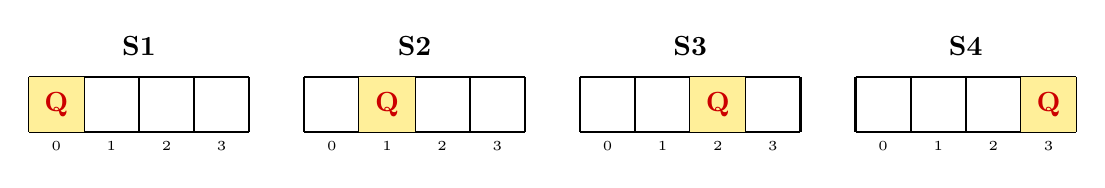
\begin{tikzpicture}[scale=0.7]
  \foreach \s/\c/\xoff in {S1/0/0, S2/1/5, S3/2/10, S4/3/15}{
    \begin{scope}[xshift=\xoff cm]
      \draw[step=1, thick] (0,0) grid (4,1);
      \fill[queencol!40] (\c, 0) rectangle (\c+1, 1);
      \node[font=\bfseries] at (\c+0.5, 0.5) {\textcolor{myred}{Q}};
      \node[above] at (2, 1.2) {\textbf{\s}};
      \foreach \i in {0,...,3}{ \node[below, font=\tiny] at (\i+0.5, 0) {\i}; }
    \end{scope}
  }
\end{tikzpicture}
\end{center}

第 0 行结束后：\textbf{4 个状态}，每个计数 $= 1$。

%--- Row 1 ---
\subsection{第 1 行}

对第 0 行产生的每个状态，计算可用列并放置皇后。

\begin{stepbox}[S1: $(C=\{0\},\; D_\searrow=\{1\},\; D_\nearrow=\emptyset)$]
可用列 $= \{0,1,2,3\} \setminus \{0\} \setminus \{1\} \setminus \emptyset = \{2, 3\}$

\textbf{Q 在列 2}：
\begin{itemize}[nosep]
  \item $C = \{0,2\}$
  \item $D_\searrow$: $\{1\} \cup \{2\} = \{1,2\} \xrightarrow{\text{右移}} \{2,3\}$
  \item $D_\nearrow$: $\emptyset \cup \{2\} = \{2\} \xrightarrow{\text{左移}} \{1\}$
  \item 新状态 $(\{0,2\},\;\{2,3\},\;\{1\})$
\end{itemize}

\textbf{Q 在列 3}：
\begin{itemize}[nosep]
  \item $C = \{0,3\}$
  \item $D_\searrow$: $\{1\} \cup \{3\} = \{1,3\} \xrightarrow{\text{右移}} \{2\}$ \ \small（$3\!+\!1\!=\!4$ 超出棋盘）
  \item $D_\nearrow$: $\emptyset \cup \{3\} = \{3\} \xrightarrow{\text{左移}} \{2\}$
  \item 新状态 $(\{0,3\},\;\{2\},\;\{2\})$
\end{itemize}
\end{stepbox}

\begin{stepbox}[S2: $(C=\{1\},\; D_\searrow=\{2\},\; D_\nearrow=\{0\})$]
可用列 $= \{0,1,2,3\} \setminus \{1\} \setminus \{2\} \setminus \{0\} = \{3\}$

\textbf{Q 在列 3}：
\begin{itemize}[nosep]
  \item $C = \{1,3\}$
  \item $D_\searrow$: $\{2\} \cup \{3\} = \{2,3\} \xrightarrow{\text{右移}} \{3\}$ \ \small（$3\!+\!1\!=\!4$ 超出）
  \item $D_\nearrow$: $\{0\} \cup \{3\} = \{0,3\} \xrightarrow{\text{左移}} \{2\}$ \ \small（$0\!-\!1\!=\!-1$ 超出）
  \item 新状态 $(\{1,3\},\;\{3\},\;\{2\})$
\end{itemize}
\end{stepbox}

\begin{stepbox}[S3: $(C=\{2\},\; D_\searrow=\{3\},\; D_\nearrow=\{1\})$]
可用列 $= \{0,1,2,3\} \setminus \{2\} \setminus \{3\} \setminus \{1\} = \{0\}$

\textbf{Q 在列 0}：
\begin{itemize}[nosep]
  \item $C = \{0,2\}$
  \item $D_\searrow$: $\{3\} \cup \{0\} = \{0,3\} \xrightarrow{\text{右移}} \{1\}$ \ \small（$3\!+\!1$ 超出）
  \item $D_\nearrow$: $\{1\} \cup \{0\} = \{0,1\} \xrightarrow{\text{左移}} \{0\}$ \ \small（$0\!-\!1$ 超出）
  \item 新状态 $(\{0,2\},\;\{1\},\;\{0\})$
\end{itemize}
\end{stepbox}

\begin{stepbox}[S4: $(C=\{3\},\; D_\searrow=\emptyset,\; D_\nearrow=\{2\})$]
可用列 $= \{0,1,2,3\} \setminus \{3\} \setminus \emptyset \setminus \{2\} = \{0, 1\}$

\textbf{Q 在列 0}：
\begin{itemize}[nosep]
  \item $C = \{0,3\}$
  \item $D_\searrow$: $\emptyset \cup \{0\} = \{0\} \xrightarrow{\text{右移}} \{1\}$
  \item $D_\nearrow$: $\{2\} \cup \{0\} = \{0,2\} \xrightarrow{\text{左移}} \{1\}$ \ \small（$0\!-\!1$ 超出）
  \item 新状态 $(\{0,3\},\;\{1\},\;\{1\})$
\end{itemize}

\textbf{Q 在列 1}：
\begin{itemize}[nosep]
  \item $C = \{1,3\}$
  \item $D_\searrow$: $\emptyset \cup \{1\} = \{1\} \xrightarrow{\text{右移}} \{2\}$
  \item $D_\nearrow$: $\{2\} \cup \{1\} = \{1,2\} \xrightarrow{\text{左移}} \{0,1\}$
  \item 新状态 $(\{1,3\},\;\{2\},\;\{0,1\})$
\end{itemize}
\end{stepbox}

\begin{center}
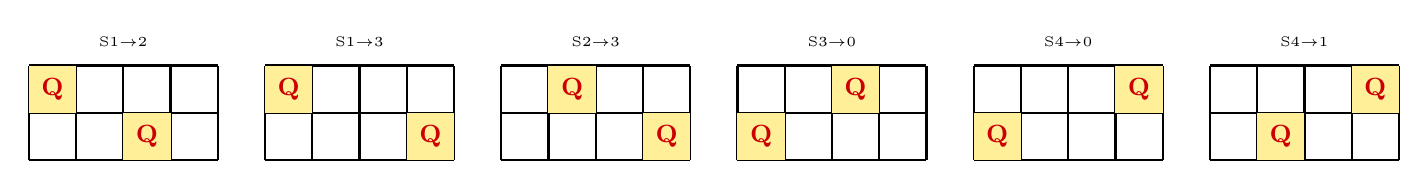
\begin{tikzpicture}[scale=0.6]
  \foreach \s/\ca/\cb/\xoff [count=\n] in {
    {S1$\to$2}/0/2/0, {S1$\to$3}/0/3/5, {S2$\to$3}/1/3/10,
    {S3$\to$0}/2/0/15, {S4$\to$0}/3/0/20, {S4$\to$1}/3/1/25}{
    \begin{scope}[xshift=\xoff cm]
      \draw[step=1, thick] (0,0) grid (4,2);
      \fill[queencol!40] (\ca, 1) rectangle (\ca+1, 2);
      \fill[queencol!40] (\cb, 0) rectangle (\cb+1, 1);
      \node[font=\small\bfseries] at (\ca+0.5, 1.5) {\textcolor{myred}{Q}};
      \node[font=\small\bfseries] at (\cb+0.5, 0.5) {\textcolor{myred}{Q}};
      \node[above, font=\tiny] at (2, 2.2) {\s};
    \end{scope}
  }
\end{tikzpicture}
\end{center}

第 1 行结束后：\textbf{6 个状态}，每个计数 $= 1$。

%--- Row 2 ---
\subsection{第 2 行}

\begin{stepbox}[状态 1: $(\{0,2\},\;\{2,3\},\;\{1\})$ --- 来自 S1$\to$列2]
可用列 $= \{0,1,2,3\} \setminus \{0,2\} \setminus \{2,3\} \setminus \{1\} = \emptyset$

\textcolor{myred}{\textbf{死胡同！}} 无列可放。此分支终止。
\end{stepbox}

\begin{stepbox}[状态 2: $(\{0,3\},\;\{2\},\;\{2\})$ --- 来自 S1$\to$列3]
可用列 $= \{0,1,2,3\} \setminus \{0,3\} \setminus \{2\} \setminus \{2\} = \{1\}$

\textbf{Q 在列 1}：
\begin{itemize}[nosep]
  \item $C = \{0,1,3\}$
  \item $D_\searrow$: $\{2\} \cup \{1\} = \{1,2\} \xrightarrow{\text{右移}} \{2,3\}$
  \item $D_\nearrow$: $\{2\} \cup \{1\} = \{1,2\} \xrightarrow{\text{左移}} \{0,1\}$
  \item 新状态 $(\{0,1,3\},\;\{2,3\},\;\{0,1\})$
\end{itemize}
\end{stepbox}

\begin{stepbox}[状态 3: $(\{1,3\},\;\{3\},\;\{2\})$ --- 来自 S2$\to$列3]
可用列 $= \{0,1,2,3\} \setminus \{1,3\} \setminus \{3\} \setminus \{2\} = \{0\}$

\textbf{Q 在列 0}：
\begin{itemize}[nosep]
  \item $C = \{0,1,3\}$
  \item $D_\searrow$: $\{3\} \cup \{0\} = \{0,3\} \xrightarrow{\text{右移}} \{1\}$ \ \small（$3\!+\!1$ 超出）
  \item $D_\nearrow$: $\{2\} \cup \{0\} = \{0,2\} \xrightarrow{\text{左移}} \{1\}$ \ \small（$0\!-\!1$ 超出）
  \item 新状态 $(\{0,1,3\},\;\{1\},\;\{1\})$
\end{itemize}
\end{stepbox}

\begin{stepbox}[状态 4: $(\{0,2\},\;\{1\},\;\{0\})$ --- 来自 S3$\to$列0]
可用列 $= \{0,1,2,3\} \setminus \{0,2\} \setminus \{1\} \setminus \{0\} = \{3\}$

\textbf{Q 在列 3}：
\begin{itemize}[nosep]
  \item $C = \{0,2,3\}$
  \item $D_\searrow$: $\{1\} \cup \{3\} = \{1,3\} \xrightarrow{\text{右移}} \{2\}$ \ \small（$3\!+\!1$ 超出）
  \item $D_\nearrow$: $\{0\} \cup \{3\} = \{0,3\} \xrightarrow{\text{左移}} \{2\}$ \ \small（$0\!-\!1$ 超出）
  \item 新状态 $(\{0,2,3\},\;\{2\},\;\{2\})$
\end{itemize}
\end{stepbox}

\begin{stepbox}[状态 5: $(\{0,3\},\;\{1\},\;\{1\})$ --- 来自 S4$\to$列0]
可用列 $= \{0,1,2,3\} \setminus \{0,3\} \setminus \{1\} \setminus \{1\} = \{2\}$

\textbf{Q 在列 2}：
\begin{itemize}[nosep]
  \item $C = \{0,2,3\}$
  \item $D_\searrow$: $\{1\} \cup \{2\} = \{1,2\} \xrightarrow{\text{右移}} \{2,3\}$
  \item $D_\nearrow$: $\{1\} \cup \{2\} = \{1,2\} \xrightarrow{\text{左移}} \{0,1\}$
  \item 新状态 $(\{0,2,3\},\;\{2,3\},\;\{0,1\})$
\end{itemize}
\end{stepbox}

\begin{stepbox}[状态 6: $(\{1,3\},\;\{2\},\;\{0,1\})$ --- 来自 S4$\to$列1]
可用列 $= \{0,1,2,3\} \setminus \{1,3\} \setminus \{2\} \setminus \{0,1\} = \emptyset$

\textcolor{myred}{\textbf{死胡同！}} 无列可放。此分支终止。
\end{stepbox}

第 2 行结束后：\textbf{4 个存活状态}（2 个死胡同被剪枝）。

\begin{center}
\renewcommand{\arraystretch}{1.3}
\begin{tabular}{c|c|c|l}
\toprule
编号 & 状态 $(C, D_\searrow, D_\nearrow)$ & 计数 & 路径 \\
\midrule
R2-1 & $(\{0,1,3\},\;\{2,3\},\;\{0,1\})$ & 1 & 行0:列0 $\to$ 行1:列3 $\to$ 行2:列1 \\
R2-2 & $(\{0,1,3\},\;\{1\},\;\{1\})$ & 1 & 行0:列1 $\to$ 行1:列3 $\to$ 行2:列0 \\
R2-3 & $(\{0,2,3\},\;\{2\},\;\{2\})$ & 1 & 行0:列2 $\to$ 行1:列0 $\to$ 行2:列3 \\
R2-4 & $(\{0,2,3\},\;\{2,3\},\;\{0,1\})$ & 1 & 行0:列3 $\to$ 行1:列0 $\to$ 行2:列2 \\
\bottomrule
\end{tabular}
\end{center}

%--- Row 3 ---
\subsection{第 3 行（最后一行）}

\begin{stepbox}[R2-1: $(\{0,1,3\},\;\{2,3\},\;\{0,1\})$]
可用列 $= \{0,1,2,3\} \setminus \{0,1,3\} \setminus \{2,3\} \setminus \{0,1\} = \emptyset$

唯一空缺列 2 被 $D_\searrow$ 阻挡。\textcolor{myred}{\textbf{死胡同！}}
\end{stepbox}

\begin{stepbox}[R2-2: $(\{0,1,3\},\;\{1\},\;\{1\})$]
可用列 $= \{0,1,2,3\} \setminus \{0,1,3\} \setminus \{1\} \setminus \{1\} = \{2\}$

\textbf{Q 在列 2}：$C = \{0,1,2,3\}$ --- 所有列已满！

\textcolor{mygreen}{\textbf{有效解！}} 路径：行0:列1, 行1:列3, 行2:列0, 行3:列2。

\begin{center}
\begin{tikzpicture}[scale=0.8]
  \foreach \r/\c in {0/1, 1/3, 2/0, 3/2}{
    \fill[queencol!40] (\c, 3-\r) rectangle (\c+1, 4-\r);
  }
  \draw[step=1, thick] (0,0) grid (4,4);
  \foreach \r/\c in {0/1, 1/3, 2/0, 3/2}{
    \node[font=\Large\bfseries] at (\c+0.5, 3.5-\r) {\textcolor{myred}{Q}};
  }
  \foreach \i in {0,...,3}{
    \node[left, font=\small] at (0, 3.5-\i) {行\i};
    \node[below, font=\small] at (\i+0.5, 0) {列\i};
  }
  \node[right, font=\large, mygreen] at (4.5, 2) {\textbf{解 1}};
\end{tikzpicture}
\end{center}
\end{stepbox}

\begin{stepbox}[R2-3: $(\{0,2,3\},\;\{2\},\;\{2\})$]
可用列 $= \{0,1,2,3\} \setminus \{0,2,3\} \setminus \{2\} \setminus \{2\} = \{1\}$

\textbf{Q 在列 1}：$C = \{0,1,2,3\}$ --- 所有列已满！

\textcolor{mygreen}{\textbf{有效解！}} 路径：行0:列2, 行1:列0, 行2:列3, 行3:列1。

\begin{center}
\begin{tikzpicture}[scale=0.8]
  \foreach \r/\c in {0/2, 1/0, 2/3, 3/1}{
    \fill[queencol!40] (\c, 3-\r) rectangle (\c+1, 4-\r);
  }
  \draw[step=1, thick] (0,0) grid (4,4);
  \foreach \r/\c in {0/2, 1/0, 2/3, 3/1}{
    \node[font=\Large\bfseries] at (\c+0.5, 3.5-\r) {\textcolor{myred}{Q}};
  }
  \foreach \i in {0,...,3}{
    \node[left, font=\small] at (0, 3.5-\i) {行\i};
    \node[below, font=\small] at (\i+0.5, 0) {列\i};
  }
  \node[right, font=\large, mygreen] at (4.5, 2) {\textbf{解 2}};
\end{tikzpicture}
\end{center}
\end{stepbox}

\begin{stepbox}[R2-4: $(\{0,2,3\},\;\{2,3\},\;\{0,1\})$]
可用列 $= \{0,1,2,3\} \setminus \{0,2,3\} \setminus \{2,3\} \setminus \{0,1\} = \emptyset$

唯一空缺列 1 被 $D_\nearrow$ 阻挡。\textcolor{myred}{\textbf{死胡同！}}
\end{stepbox}

%=============================================================================
\section{结果汇总}
%=============================================================================

\subsection{搜索树总览}

\begin{center}
\begin{tikzpicture}[
  level distance=2.2cm, sibling distance=3.5cm,
  edge from parent/.style={draw, thick, -Stealth},
  every node/.style={font=\small},
  dead/.style={text=myred, font=\small\itshape},
  sol/.style={text=mygreen, font=\small\bfseries},
  grow=down
]
\node {初始}
  child { node {列0}
    child { node {列2}
      child { node[dead] {$\emptyset$ 死} edge from parent node[left,font=\tiny] {行2} }
      edge from parent node[left,font=\tiny] {行1}
    }
    child { node {列3}
      child { node {列1}
        child { node[sol] {列2 {\Large$\checkmark$}} edge from parent node[left,font=\tiny] {行3} }
        edge from parent node[left,font=\tiny] {行2}
      }
      edge from parent node[right,font=\tiny] {行1}
    }
    edge from parent node[left,font=\tiny] {行0}
  }
  child { node {列1}
    child { node {列3}
      child { node {列0}
        child { node[sol] {列2 {\Large$\checkmark$}} edge from parent node[left,font=\tiny] {行3} }
        edge from parent node[left,font=\tiny] {行2}
      }
      edge from parent node[left,font=\tiny] {行1}
    }
    edge from parent node[left,font=\tiny] {行0}
  }
  child { node {列2}
    child { node {列0}
      child { node {列3}
        child { node[sol] {列1 {\Large$\checkmark$}} edge from parent node[left,font=\tiny] {行3} }
        edge from parent node[left,font=\tiny] {行2}
      }
      edge from parent node[left,font=\tiny] {行1}
    }
    edge from parent node[left,font=\tiny] {行0}
  }
  child { node {列3}
    child { node {列0}
      child { node {列2}
        child { node[dead] {$\emptyset$ 死} edge from parent node[left,font=\tiny] {行3} }
        edge from parent node[left,font=\tiny] {行2}
      }
      edge from parent node[left,font=\tiny] {行1}
    }
    child { node {列1}
      child { node[dead] {$\emptyset$ 死} edge from parent node[left,font=\tiny] {行2} }
      edge from parent node[left,font=\tiny] {行1}
    }
    edge from parent node[right,font=\tiny] {行0}
  };
\end{tikzpicture}
\end{center}

\subsection{统计}

\begin{center}
\renewcommand{\arraystretch}{1.3}
\begin{tabular}{l|c}
\toprule
\textbf{指标} & \textbf{值} \\
\midrule
第 0 行后状态数 & 4 \\
第 1 行后状态数 & 6 \\
第 2 行后存活状态数 & 4（2 个死胡同） \\
第 3 行后存活状态数 & 2（2 个死胡同） \\
\midrule
\textbf{总解数} $Z_4$ & $\boldsymbol{2}$ \\
\bottomrule
\end{tabular}
\end{center}

\subsection{验证两个解}

\begin{sumbox}[解 1 验证：行0:列1, 行1:列3, 行2:列0, 行3:列2]
\textbf{行约束}：每行恰好 1 个 \checkmark \\
\textbf{列约束}：$\{0,1,2,3\}$ 各出现一次 \checkmark \\
\textbf{$\searrow$ 对角线}：皇后所在对角线编号 $(i\!-\!j)$: $-1, -2, 2, 1$，互不相同 \checkmark \\
\textbf{$\nearrow$ 对角线}：皇后所在反对角线编号 $(i\!+\!j)$: $1, 4, 2, 5$，互不相同 \checkmark
\end{sumbox}

\begin{sumbox}[解 2 验证：行0:列2, 行1:列0, 行2:列3, 行3:列1]
\textbf{行约束}：每行恰好 1 个 \checkmark \\
\textbf{列约束}：$\{0,1,2,3\}$ 各出现一次 \checkmark \\
\textbf{$\searrow$ 对角线}：$(i\!-\!j)$: $-2, 1, -1, 2$，互不相同 \checkmark \\
\textbf{$\nearrow$ 对角线}：$(i\!+\!j)$: $2, 1, 5, 4$，互不相同 \checkmark
\end{sumbox}

\begin{notebox}[对称性]
解 1 和解 2 互为左右镜像：将棋盘沿纵轴翻转（列 $j \to 3-j$），解 1 变为解 2。
这是 $4\times 4$ 皇后问题仅有的对称性。
\end{notebox}

%=============================================================================
\section{用 $A$ 矩阵语言验证解 1}
%=============================================================================

最后，我们用 $A$ 矩阵的原始定义，\textbf{逐条约束线}验证解 1 的分区函数贡献为 1。

解 1 的棋盘配置 $\sigma$：
\[
\sigma = \begin{pmatrix}
0 & 1 & 0 & 0 \\
0 & 0 & 0 & 1 \\
1 & 0 & 0 & 0 \\
0 & 0 & 1 & 0
\end{pmatrix}
\quad \text{（$\sigma_{ij} = 1$ 表示 $(i,j)$ 有皇后）}
\]

\subsection{行约束（$\bv{v}_0 \cdot A^4 \cdot \bv{v}_1^T$，要求恰好 1 个）}

\begin{exbox}[4 条行约束]
\textbf{行 0}：$\sigma = (0,1,0,0)$
\[
(1,0) \xrightarrow{A(0)} (1,0) \xrightarrow{A(1)} (0,1) \xrightarrow{A(0)} (0,1) \xrightarrow{A(0)} (0,1) \cdot \binom{0}{1} = 1 \quad \checkmark
\]
\textbf{行 1}：$\sigma = (0,0,0,1)$
\[
(1,0) \xrightarrow{A(0)} (1,0) \xrightarrow{A(0)} (1,0) \xrightarrow{A(0)} (1,0) \xrightarrow{A(1)} (0,1) \cdot \binom{0}{1} = 1 \quad \checkmark
\]
\textbf{行 2}：$\sigma = (1,0,0,0)$
\[
(1,0) \xrightarrow{A(1)} (0,1) \xrightarrow{A(0)} (0,1) \xrightarrow{A(0)} (0,1) \xrightarrow{A(0)} (0,1) \cdot \binom{0}{1} = 1 \quad \checkmark
\]
\textbf{行 3}：$\sigma = (0,0,1,0)$
\[
(1,0) \xrightarrow{A(0)} (1,0) \xrightarrow{A(0)} (1,0) \xrightarrow{A(1)} (0,1) \xrightarrow{A(0)} (0,1) \cdot \binom{0}{1} = 1 \quad \checkmark
\]
\end{exbox}

\subsection{列约束（$\bv{v}_0 \cdot A^4 \cdot \bv{v}_1^T$，要求恰好 1 个）}

\begin{exbox}[4 条列约束]
\textbf{列 0}：从上到下 $\sigma = (0,0,1,0)$
\[
(1,0) \xrightarrow{A(0)} (1,0) \xrightarrow{A(0)} (1,0) \xrightarrow{A(1)} (0,1) \xrightarrow{A(0)} (0,1) \cdot \binom{0}{1} = 1 \quad \checkmark
\]
\textbf{列 1}：$\sigma = (1,0,0,0)$
\[
(1,0) \xrightarrow{A(1)} (0,1) \xrightarrow{A(0)} (0,1) \xrightarrow{A(0)} (0,1) \xrightarrow{A(0)} (0,1) \cdot \binom{0}{1} = 1 \quad \checkmark
\]
\textbf{列 2}：$\sigma = (0,0,0,1)$ \quad 同行 1 的计算 $= 1$ \quad \checkmark \\[3pt]
\textbf{列 3}：$\sigma = (0,1,0,0)$ \quad 同行 0 的计算 $= 1$ \quad \checkmark
\end{exbox}

\subsection{$\searrow$ 对角线约束（$\bv{v}_0 \cdot A^L \cdot \bv{v}_2^T$，至多 1 个）}

$4\times 4$ 棋盘有 7 条 $\searrow$ 对角线，长度分别为 $1, 2, 3, 4, 3, 2, 1$。

\begin{exbox}[$\searrow$ 对角线验证]
对角线编号 $d = i - j$：
\begin{itemize}[nosep]
  \item $d = -3$：仅 $(0,3)$，$\sigma=0$。$\;(1,0)\cdot A(0)\cdot(1,1)^T = 1$ \checkmark
  \item $d = -2$：$(0,2),(1,3)$，$\sigma=(0,1)$。$(1,0)\!\cdot\! A(0)\!\cdot\! A(1)\!\cdot\!(1,1)^T = (0,1)\!\cdot\!(1,1)^T=1$ \checkmark
  \item $d = -1$：$(0,1),(1,2),(2,3)$，$\sigma=(1,0,0)$。$(1,0)\!\cdot\! A(1)\!\cdot\! A(0)^2\!\cdot\!(1,1)^T = (0,1)\!\cdot\!(1,1)^T=1$ \checkmark
  \item $d = 0$：主对角线 $(0,0),(1,1),(2,2),(3,3)$，$\sigma=(0,0,0,0)$。$(1,0)\!\cdot\! A(0)^4\!\cdot\!(1,1)^T = (1,0)\!\cdot\!(1,1)^T=1$ \checkmark
  \item $d = 1$：$(1,0),(2,1),(3,2)$，$\sigma=(0,0,1)$。$(1,0)\!\cdot\! A(0)^2\!\cdot\! A(1)\!\cdot\!(1,1)^T = (0,1)\!\cdot\!(1,1)^T=1$ \checkmark
  \item $d = 2$：$(2,0),(3,1)$，$\sigma=(1,0)$。$(1,0)\!\cdot\! A(1)\!\cdot\! A(0)\!\cdot\!(1,1)^T = (0,1)\!\cdot\!(1,1)^T=1$ \checkmark
  \item $d = 3$：仅 $(3,0)$，$\sigma=0$。$\;(1,0)\cdot A(0)\cdot(1,1)^T = 1$ \checkmark
\end{itemize}
\end{exbox}

\subsection{$\nearrow$ 对角线约束}

同理，7 条 $\nearrow$ 对角线（编号 $s = i+j$）：

\begin{exbox}[$\nearrow$ 对角线验证]
\begin{itemize}[nosep]
  \item $s = 0$：仅 $(0,0)$，$\sigma=0$ $\to$ $1$ \checkmark
  \item $s = 1$：$(0,1),(1,0)$，$\sigma=(1,0)$ $\to$ $(0,1)\cdot(1,1)^T=1$ \checkmark
  \item $s = 2$：$(0,2),(1,1),(2,0)$，$\sigma=(0,0,1)$ $\to$ $1$ \checkmark
  \item $s = 3$：$(0,3),(1,2),(2,1),(3,0)$，$\sigma=(0,0,0,0)$ $\to$ $(1,0)\cdot(1,1)^T=1$ \checkmark
  \item $s = 4$：$(1,3),(2,2),(3,1)$，$\sigma=(1,0,0)$ $\to$ $1$ \checkmark
  \item $s = 5$：$(2,3),(3,2)$，$\sigma=(0,1)$ $\to$ $1$ \checkmark
  \item $s = 6$：仅 $(3,3)$，$\sigma=0$ $\to$ $1$ \checkmark
\end{itemize}
\end{exbox}

\subsection{分区函数贡献}

解 1 对分区函数的贡献：
\[
\text{val} = \underbrace{1 \times 1 \times 1 \times 1}_{\text{4 行}} \times \underbrace{1 \times 1 \times 1 \times 1}_{\text{4 列}} \times \underbrace{1^7}_{\searrow\text{对角线}} \times \underbrace{1^7}_{\nearrow\text{对角线}} = 1
\]

同理，解 2 的贡献也是 1。其余所有 $2^{16} - 2$ 种配置的贡献均为 0。

\begin{keybox}[最终结果]
\[
\boxed{Z_4 = \sum_{\text{所有 } 2^{16} \text{ 种配置}} \text{val}(\sigma) = 1 + 1 + 0 + \cdots + 0 = 2}
\]
\end{keybox}

%=============================================================================
\section{回顾与总结}
%=============================================================================

\begin{sumbox}[完整计算流程回顾]
\begin{enumerate}
  \item \textbf{构件}：$A$ 矩阵 $\begin{pmatrix}\hat{n}_0 & \hat{n}_1 \\ 0 & \hat{n}_0\end{pmatrix}$ 编码「至多/恰好 1 个」约束
  \item \textbf{T 张量}：每个格点 4 条约束线的 $A$ 矩阵元相乘，得到 17 个非零元
  \item \textbf{边界}：$\bv{v}_0$ 启动信号，$\bv{v}_1$（恰好1个）或 $\bv{v}_2$（至多1个）终止
  \item \textbf{逐行收缩}：跟踪列/对角线信号，对角线信号每行移位
  \item \textbf{结果}：4 行遍历后，恰好 2 个状态存活 → $Z_4 = 2$
\end{enumerate}
\end{sumbox}

\end{document}
